\section{Maximum Margin Classifiers}

\mode<presentation>{
\begin{frame} 
    \begin{center} \huge
        \secname
    \end{center}
    \begin{center}
     What is a \emph{margin} and why should we care about maximizing it?   
    \end{center}
\end{frame}
}

\subsection{The margin}

\begin{frame}\frametitle{Identifying the margin}
\mode<article>{
Consider the following linearly separable binary classification problem and the different hyperplanes for separating the two classes. In order to identify the margn of a hyperplane:
}

\only<1-3>{
\begin{enumerate}[(a)]
\item select a hyperplane,
\item select the traninng point closest to the hyperplane. Call it $\vec x^{*}$. $\vec x^{*}$ has the shortest normal distance to the hyperplane.
\item measure the normal distance between $\vec x^{*}$ and the hyperplane and call it $d_{w}$
\end{enumerate}
}
%\begin{figure}[h]
    %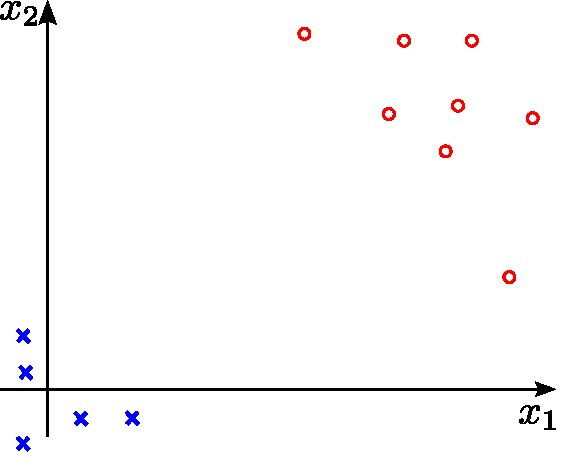
\includegraphics[width=0.5\linewidth]{img/section2_fig13_v2_nomargin_h_none}
    %\mode<article>{
    %\caption{Different hyperplanes for a linearly separable problem.}
    %}
%\end{figure}

\begin{figure}[ht]
     \centering
     \savebox{\imagebox}{
	 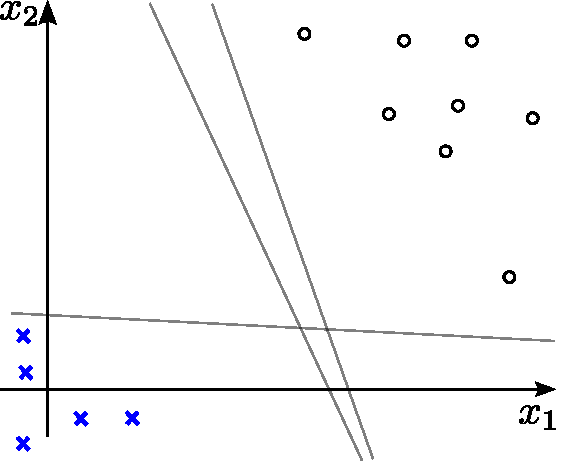
\includegraphics[width=0.35\textwidth]{img/section2_fig13_v2_nomargin_h_multiple}}%
     \only<1>{
     \begin{subfigure}[t]{0.35\textwidth}
         \centering
         \usebox{\imagebox}% Place largest image
         \mode<article>{
         \caption{}
         }
         \label{fig:multiplehyperplanes}
     \end{subfigure}
     }
     \hspace{2mm}
     \only<2>{
     \begin{subfigure}[t]{0.35\textwidth}
         \centering
         \raisebox{\dimexpr.5\ht\imagebox-.5\height}{% Raise smaller image into place
         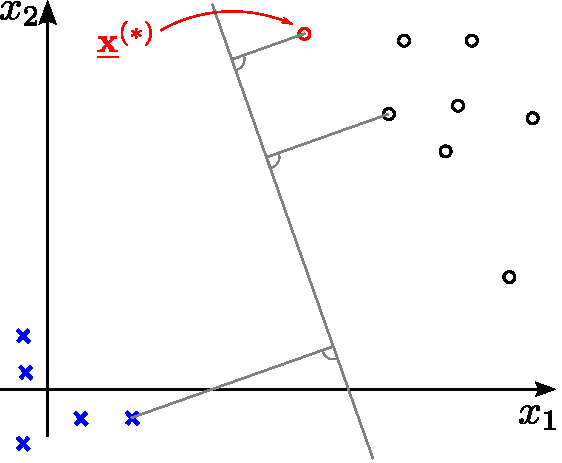
\includegraphics[width=0.99\textwidth]{img/section2_fig13_v2_nomargin_h_closest}
         }
         \mode<article>{
         \caption{}
         }
     \end{subfigure}
     }
     \hspace{2mm}
     \only<3,4>{
     \begin{subfigure}[t]{0.35\textwidth}
         \centering
         \raisebox{\dimexpr.5\ht\imagebox-.5\height}{% Raise smaller image into place
         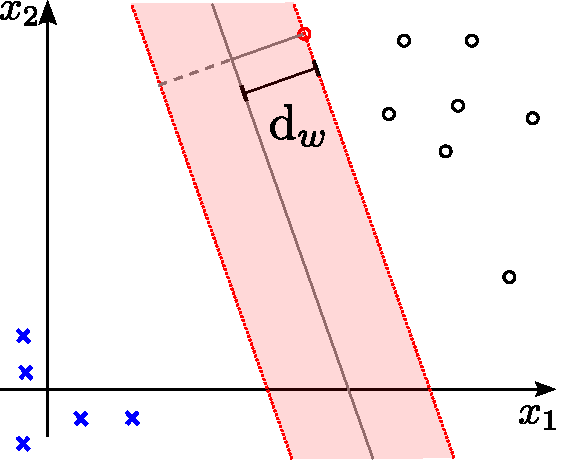
\includegraphics[width=0.99\textwidth]{img/section2_fig13_v2_nomargin_h_margin}
         }
         \mode<article>{
         \caption{}
         }
         \label{fig:margin}
     \end{subfigure}
     \hspace{2mm}
     }
     \only<4>{
     \begin{subfigure}[t]{0.35\textwidth}
         \centering
         \raisebox{\dimexpr.5\ht\imagebox-.5\height}{% Raise smaller image into place
         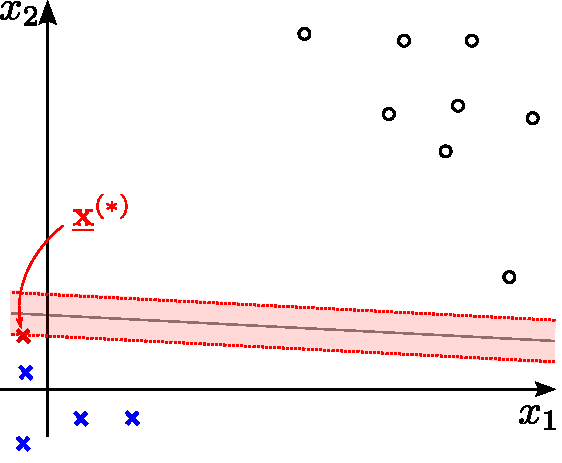
\includegraphics[width=0.99\textwidth]{img/section2_fig13_v2_nomargin_h_marginother}
         }
         \mode<article>{
         \caption{}
         }
         \label{fig:marginother}
     \end{subfigure}
     }
     \mode<article>{
     \caption{Identifying the margin $d_{w}$ for a hyperplane.}
	 }
	 \label{fig:identifymargin}
\end{figure}

The distance $d_{w}$ is the \emph{margin} for that hyperplane.

\question{What are the implications of a wide vs. narrow margin?}

    
\end{frame}

\begin{frame}\frametitle{Wide vs. narrow margins}

Different hyperplanes may score the same value on the error functions and produce identical predictions on the training set.
    
\end{frame}

\begin{frame}

      The {\em margin} is the smallest distance between a separating hyperplane and a training sample. We will refer to the training sample closest to the decision boundary as $\vec x^{(*)}$.\\
            Separating the training data with a larger margin is more likely to reduce classification error on unseen data (i.e. lower generalization error, less overfitting).
            A simplisitc justification for this: \\
            Assume we have found the separating hyperplane with the maximum margin for perfectly separable data. From this:
            \begin{enumerate}[(1)]
                \item The distance between the classes is at least twice as wide as the distance from the hyperplane to $\vec x^{(*)}$.
                \item An unseen pattern $\vec x_{(test)}$ is more likely to land closer to training patterns of the same class than patterns from the other class.
                \item The distance between $\vec x_{(test)}$ and $\vec x^{(*)}$ is more likely to be larger than the margin if the points belong to different classes and more likely to be below the margin if both belong to the same class.
            \end{enumerate}
            Another way to look at this:\\
            Consider a second hyperplane with the same orientation $\vec w$ but less than maximum (i.e. more narrow) margin. Shift the second hyperplane so that our sample $\vec x^{(*)}$ also lies on the margin of the second hyperplane. The shifting results in the decision boundaries of both hypeplanes appearing parallel to one another, both make contact with $\vec x^{(*)}$. The difference is that the hyperplane with the smaller margin appears to lie inside the first hyperplane. Now consider an unseen pattern $\vec x_{(test)}$ that is very similar to $\vec x^{(*)}$ (i.e. $\vec x_{(test)} = \vec x^{(*)} + \vec {noise}$). $\vec x_{(test)}$ belongs to the same class as $\vec x^{(*)}$. The noise can result in the $\vec x_{(test)}$ falling inside the margin of the first hyperplane. Because the margin of the second hyperplane is more narrow, the decision boundary of that plane is closer to $\vec x^{(*)}$. This means that $\vec x_{(test)}$ is more likely to fall on the wrong side of the second decision boundary and get misclassified (i.e. higher generlization error). This is less likely to happen for the first hypeplane because the mazimum margin pushes the decision boundary away from the $\vec x^{(*)}$. We would need to apply more noise on $\vec x_{(test)}$  until it gets misclassified by the maximum margin hyperplane.\vspace{5cm}
            \textit{Where does the VC dimension come into all of this?}\\
            Large margins imply small VC dimension, because a lrger margin tightens the upper bound of the VC dimension, regardless of the dimensionality of the problem. Vapnik's theorem tells us\\
            $$
                d_{VC} \quad\leq\quad \min \bigg( \bigg\lfloor 
                \frac{\mathrm{d}_R^2}{\mathrm{d}_{{w}}^2}
            \bigg\rfloor, N \bigg) + 1
            $$\\
            where,\\
            \begin{tabular}{rl}
                $N$\;:& dimension of feature space \\[1mm]
                $\mathrm{d}_w$\;:& the margin: 
                    $\frac{1}{\|\vec w \|} \geq \mathrm{d}_w$ \\[1mm]
                $\mathrm{d}_R$\;:& radius of a sphere containing all training points
            \end{tabular}\\
            This bound basically tells us that if we draw a sphere around our training data and a second sphere inside of it using the margin as its radius. Knowing that the innner sphere can be placed in the center and not contain any samples. The theorem then tells us that the VC-dimension is no longer $N+1$ but only as big as the integer component of the ratio $\frac{\mathrm{d}_R^2}{\mathrm{d}_{{w}}^2}$.
            
\end{frame}
